\subsection{Nonlinear Model Predictive Control}
\label{sec::312_nmpc}
At the heart of nonlinear model predictive control stands sequential quadratic programming. Before we come to the actual problem formulation, we need to understand how sequential quadratic programming can be used to solve nonlinear optimization problems. We will then come to recognize that if we can find a canonical formulation of our problem, it will become possible to apply sequential quadratic programming to it. The next paragraph - Sequential Quadratic Programming, will therefore shortly introduce the reader to the desired method that will be used to solve the  nonlinear optimization problem, while the subsequent paragraph - Canonical Formulation of Nonlinear Model Predictive Control, will then explain how to fit humanoid walking into this framework.
\subsubsection{Sequential Quadratic Programming}
\label{sec::312_sqp}
Sequential quadratic programming is a powerful concept to solve nonlinearly constrained optimization problems. The nonlinear programming problem to be solved is of the form
\begin{align}
	\min_{\bm{x}}\, &f(\bm{x})
	\label{eq::312_objective}\\
	\text{subject to: } &\bm{h}(\bm{x}) = \bm{0}\\
	&\bm{g}(\bm{x}) \leq \bm{0},
\end{align}
where $f:\,\mathbb{R}^N\rightarrow\mathbb{R}$, $\bm{h}:\,\mathbb{R}^N\rightarrow\mathbb{R}^M$, and $\bm{g}:\,\mathbb{R}^N\rightarrow\mathbb{R}^P$ \cite{boggs1995sequential}. These problems arise in a variety of applications in science and include quadratic problems as special cases. The great strength of sequential quadratic programming is its ability to solve problems with nonlinear constraints, and its basic idea is to model nonlinear programming at an approximate solution $\bm{x}_k$ by a quadratic subproblem, so to find a solution to this subproblem, in order to construct a better approximation $\bm{x}_{k+1}$. Now given an objective function $f(\bm{x})$ represents a sum of squares, the problem at hand turns into a nonlinear least squares problem, and the minimization can be expressed in terms of a Gauss-Newton method \cite{schittkowski1988solving}. That is, given an objective function $f(\bm{x}) = \frac{1}{2}\bm{F}(\bm{x})^T\bm{F}(\bm{x})$, where $\bm{F}=\left(f_1,...,f_l\right)^T$, we can apply a quasi Gauss-Newton method as follows
\begin{align}
	\nabla^2f(\bm{x})\Delta\bm{x} + \nabla f(\bm{x}) = 0,
	\label{eq::312_quasi_gn}
\end{align}
where the gradient and the Hessian matrix are given as
\begin{align}
	\nabla f(\bm{x}) &= \nabla \bm{F}(\bm{x})\bm{F}(\bm{x}) \\
	\nabla^2 f(\bm{x}) &= \nabla \bm{F}(\bm{x})\nabla\bm{F}(\bm{x})^T + \bm{B}(\bm{x}).
\end{align}
Therein, $\bm{B}(\bm{x}) = \sum_1^lf_i(\bm{x})\nabla^2f_i(\bm{x})$. If we are now sufficiently close to an optimal solution $\bm{x}^*$, such that $\bm{F}(\bm{x}^*) = \left(f_1(\bm{x}^*),...,f_l(\bm{x}^*)\right)^T=\bm{0}$, we can neglect $\bm{B}(\bm{x^*})$, which turns equation \ref{eq::312_quasi_gn} into the previously stated Gauss-Newton minimization problem
\begin{align}
	\min_{\Delta\bm{x}}\,||\nabla\bm{F}(\bm{x_k})^T\Delta\bm{x}+\bm{F}(\bm{x}_k)||,
	\label{eq::312_gn_min}
\end{align}
where a new iterate is obtained by $\bm{x}_{k+1}=\bm{x}_k + \alpha_k\Delta \bm{x}$ with an appropriate step length parameter $\alpha_k$. The presented approach assures quadratic convergence, when starting sufficiently close to an optimal solution. Within the next section, we will understand how to apply this concept to control the zero moment point of a linear inverted pendulum in a balanced manner.
\subsubsection{Canonical Formulation of Nonlinear Model Predictive Control}
Not only do we want to keep a humanoid robot dynamically balanced in terms of the zero moment point, which we derived in equations \ref{eq::311_zmp_x} and \ref{eq::311_zmp_y}, but further do we want to assure this for future time steps that are yet ahead. The underlying model predictive control got first introduced in \cite{kajita2003biped}, and is based upon a linear time stepping scheme, which integrates the current jerk of the center of mass iteratively, so to estimate its future position. We will briefly present it in the following paragraph - Linear Time Stepping Scheme.
\subsubsection{Linear Time Stepping Scheme}
Suppose that the center of mass' jerk $\dddot{c}_k$ at time step $t_k$ is constant, then given the current acceleration $\ddot{c}_k$, we can obtain the acceleration $\ddot{c}_{k+1}$ at time step $t_{k+1}$ by simple integration. We can do the same for the velocity and position and therefore obtain
\begin{align}
	c_{k+1} &= \frac{T^3}{6}\dddot{c}_k+\frac{T^2}{2}\ddot{c}_k+T\dot{c}_k+c_k\\
	\dot{c}_{k+1} &= \frac{T^2}{2}\dddot{c}_k+T\ddot{c}_k+\dot{c}_k\\
	\ddot{c}_{k+1} &= T\dddot{c}_{k} + \ddot{c}_k,
\end{align}
where $T = t_{k+1}-t_k$. We can rewrite this in compact form by
\begin{align}
	&\bm{c}_{k+1} = \bm{A}\bm{c}_k + \bm{B}\dddot{c}_k \\
	&\bm{c}_{k+1} = \begin{pmatrix}
	c_{k+1} \\
	\dot{c}_{k+1} \\
	\ddot{c}_{k+1}
	\end{pmatrix},\,\,
	\bm{A} = \begin{pmatrix}
	1 & T & \frac{T^2}{2} \\
	0 & 1 & T \\
	0 & 0 & 1
	\end{pmatrix},\,\,
	\bm{B} = \begin{pmatrix}
	\frac{T^3}{6} \\
	\frac{T^2}{2} \\
	T
	\end{pmatrix}
	\label{eq::312_ltss}
\end{align}
Now by recursion, one obtains the positions, velocities, and accelerations for $n$ future time steps via
\begin{align}
	\bm{c}_{k+n} = \bm{A}^n\bm{c}_k\sum_{i=1}^n \bm{A}^{i-1}\bm{B}\dddot{c}_{k+n-i},
\end{align}
where $n\in[1,N]$. Altogether we have
\begin{align}
	\bm{A}^n = \begin{pmatrix}
	1 & nT & n^2\frac{T^2}{2} \\
	0 & 1 & nT \\
	0 & 0 & 1
	\end{pmatrix},\,\,
	\bm{A}^n\bm{B} = \begin{pmatrix}
	(1+3n+3n^2)T^3/6 \\
	(1+2n)T^2/2 \\
	T
	\end{pmatrix}.
\end{align}
The amount of time $NT$ that we predict into the future, is what we call the preview horizon. If we now concatenate the single entries of $\bm{c}_{k+n}$ for all $n\in[1,N]$ into one expression, we can relate the initial states $\bm{c}_k$ (\href{https://github.com/mhubii/nmpc_pattern_generator/blob/5a213044c927dc6aac9f7e32ce1e5fb472cd67bb/libs/pattern_generator/include/pattern_generator/base_generator.h#L140}{link}) to the states on the preview horizon in an even more compact form. With the concatenations (\href{https://github.com/mhubii/nmpc_pattern_generator/blob/5a213044c927dc6aac9f7e32ce1e5fb472cd67bb/libs/pattern_generator/include/pattern_generator/base_generator.h#L146}{link})
\begin{align}
	\bm{C}_{k+1}=\begin{pmatrix}
	c_{k+1}\\
	\vdots\\
	c_{k+N}
	\end{pmatrix},\,\,
	\dot{\bm{C}}_{k+1}=\begin{pmatrix}
	\dot{c}_{k+1}\\
	\vdots\\
	\dot{c}_{k+N}
	\end{pmatrix},\,\,
	\ddot{\bm{C}}_{k+1}=\begin{pmatrix}
	\ddot{c}_{k+1}\\
	\vdots\\
	\ddot{c}_{k+N}
	\end{pmatrix},\,\,
	\dddot{\bm{C}}_{k}=\begin{pmatrix}
	\dddot{c}_{k}\\
	\vdots\\
	\dddot{c}_{k+N-1}
	\end{pmatrix},
\end{align}
we obtain (\href{https://github.com/mhubii/nmpc_pattern_generator/blob/5a213044c927dc6aac9f7e32ce1e5fb472cd67bb/libs/pattern_generator/src/base_generator.cpp#L887}{link})
\begin{align}
	\bm{C}_{k+1} &= \bm{P}_{ps} \bm{c}_k + \bm{P}_{pu}\dddot{\bm{C}}_k
	\label{eq::312_ckp1}\\
	\dot{\bm{C}}_{k+1} &= \bm{P}_{vs} \bm{c}_k + \bm{P}_{vu}\dddot{\bm{C}}_k
	\label{eq::312_dckp1}\\
	\ddot{\bm{C}}_{k+1} &= \bm{P}_{as} \bm{c}_k + \bm{P}_{au}\dddot{\bm{C}}_k,
	\label{eq::312_ddckp1}
\end{align}
where the new matrices are given by (\href{https://github.com/mhubii/nmpc_pattern_generator/blob/5a213044c927dc6aac9f7e32ce1e5fb472cd67bb/libs/pattern_generator/src/base_generator.cpp#L403}{link})
\begin{align}
	\bm{P}_{ps} &= \begin{pmatrix}
	1 & T & T^2/2 \\
	\vdots & & \vdots \\
	1 & nT & n^2T^2/2
	\end{pmatrix},\,\,
	\bm{P}_{pu} = \begin{pmatrix}
	T^3/6 & \dots & 0 \\
	\vdots & \ddots & \vdots \\
	(1+3n+3n^2)T^2/6 & \dots & T^3/6
	\end{pmatrix} \\
	\bm{P}_{vs} &= \begin{pmatrix}
	0 & 1 & T \\
	\vdots & & \vdots \\
	0 & 1 & nT
	\end{pmatrix},\,\,
	\bm{P}_{vu} = \begin{pmatrix}
	T^2/2 & \dots & 0 \\
	\vdots & \ddots & \vdots \\
	(1+2n)/T^2/2 & \dots & T^2/2
	\end{pmatrix} \\
	\bm{P}_{as} &= \begin{pmatrix}
	0 & 0 & 1 \\
	\vdots  &  & \vdots \\
	 0 & 0 & 1
	\end{pmatrix},\,\,
	\bm{P}_{au}\begin{pmatrix}
	T & \dots & 0 \\
	\vdots & \ddots & \vdots \\
	T & \dots & T
	\end{pmatrix}.
\end{align}
If we now additionally consider the relation of the zero moment point and the center of mass, which we obtained earlier in equations \ref{eq::311_zmp_x} and \ref{eq::311_zmp_y}, we can further relate the current center of mass state to the zero moment point on the preview horizon by (\href{https://github.com/mhubii/nmpc_pattern_generator/blob/5a213044c927dc6aac9f7e32ce1e5fb472cd67bb/libs/pattern_generator/include/pattern_generator/base_generator.h#L219}{link})
\begin{align}
	\bm{Z}_{k+1} &= \bm{C}_{k+1} - \frac{c_z}{g}\ddot{\bm{C}}_{k+1} \\
	&= \left(\bm{P}_{ps}-\frac{c_z}{g}\bm{P}_{as}\right)\bm{c}_k + \left(\bm{P}_{pu}-\frac{c_z}{g}\bm{P}_{au}\right)\ddddot{\bm{C}}_k = \bm{P}_{zs} \bm{c}_k + \bm{P}_{zu}\dddot{\bm{C}}_k,
	\label{eq::312_zmp}
\end{align}
where the new matrices are given by (\href{https://github.com/mhubii/nmpc_pattern_generator/blob/5a213044c927dc6aac9f7e32ce1e5fb472cd67bb/libs/pattern_generator/src/base_generator.cpp#L420}{link})
\begin{align}
	\bm{P}_{zs} &= \begin{pmatrix}
	1 & T & T^2/2 - c_z/g \\
	\vdots & & \vdots \\
	1 & nT & n^2T^2/2 - c_z/g
	\end{pmatrix} \\ 
	\bm{P}_{zu} &= \begin{pmatrix}
	T^3/6 - Tc_z/g & \dots & 0 \\
	\vdots & \ddots & \vdots \\
	(1+3n+3n^2)T^3/6 - Tc_z/g & \dots & T^3/6-Tc_z/g
	\end{pmatrix}.
\end{align}
The expressions for the preview horizon now allow us to formulate an objective function that takes the robot's dynamic balance for future time steps into account, which in turn results in actions being taken that already take future predictions of the system's dynamics into account. The cost function will be described in the next section - The Objective Function.
\subsubsection{The Objective Function}
To create an objective function, as the one already outlined in section \ref{sec::312_sqp}, we put together squared $L^2$-norm objectives, which account for a desired reference center of mass velocity $\dot{\bm{C}}_{k+1}^\text{ref}$, a balanced foot step placement $\textbf{F}_{k+1}$ close to the zero moment point $\bm{Z}_{k+1}$, and a smooth motion for which the center of mass jerk $\dddot{\bm{C}}_{k+1}$ enters as a regularization. The objective function itself is similar to the one first introduced in \cite{herdt2010online}, but additionally takes the center of mass' rotation around the z-axis into account, and it can be written down as follows
\begin{align}
	\min_{\bm{U}_k} &\frac{\alpha}{2}||\dot{\bm{C}}^x_{k+1} - \dot{\bm{C}}_{k+1}^{x,\text{ref}}||_2^2 + \frac{\alpha}{2}||\dot{\bm{C}}^y_{k+1} - \dot{\bm{C}}_{k+1}^{y,\text{ref}}||_2^2 
	\label{eq::312_dcxy}\\
	&\frac{\alpha}{2}||\bm{E}_L\dot{\bm{F}}^{\theta,L}_{k+1} - \dot{\bm{C}}_{k+1}^{\theta,\text{ref}}||_2^2 + 	\frac{\alpha}{2}||\bm{E}_R\dot{\bm{F}}^{\theta,R}_{k+1} - \dot{\bm{C}}_{k+1}^{\theta,\text{ref}}||_2^2 
	\label{eq::312_dftheta} \\
	&\frac{\beta}{2}||\bm{Z}^x_{k+1}-\bm{F}^x_{k+1}||^2_2 + \frac{\beta}{2}||\bm{Z}^y_{k+1}-\bm{F}^y_{k+1}||^2_2 
	\label{eq::312_fxy}\\
	&\frac{\gamma}{2}||\dddot{\bm{C}}_{k+1}^x||^2_2 + \frac{\gamma}{2}||\dddot{\bm{C}}_{k+1}^y||^2_2	
	\label{eq::312_dddcxy}
\end{align}
Before we address the foot placement therein in more detail, we shortly want to highlight that the reference velocities are the commands, which enter the control loop from figure \ref{fig::31_pg}. We set them to be constant over the whole preview horizon and rotate them to the world frame  by considering the robot's current orientation (\href{https://github.com/mhubii/nmpc_pattern_generator/blob/5a213044c927dc6aac9f7e32ce1e5fb472cd67bb/libs/pattern_generator/src/base_generator.cpp#L324}{link}). When we consider that the foot cannot move once it is in contact with the ground, it becomes clear that the foot step placement must be very discrete in time. The number of steps $N_f$ that we plan for in advance is simply given by $NT/T_\text{step}$, where we just divide the duration of the preview horizon $NT$ by the time it takes to perform a step $T_\text{step}$. But as already shown in equation \ref{eq::312_zmp}, and used in equation \ref{eq::312_fxy}, we require balance on a finer timescale. We therefore project the foot placement $\tilde{\bm{F}}_k\in\mathbb{R}^{N_f\times1}$ onto the temporal resolution of the center of mass' control variable by introducing the matrices $\bm{v}_{k+1}$, $\bm{V}_{k+1}$, and the current foot position $f_k$, which yields
\begin{align}
	\bm{F}_{k+1} = \bm{v}_{k+1}f_k + \bm{V}_{k+1}\tilde{\bm{F}}_k,
	\label{eq:312_feet}
\end{align}
where $\bm{v}_{k+1}$ is a $N\times1$ matrix, and $\bm{V}_{k+1}$ is a $N\times N_f$ matrix, and they are for example for $N_f = 3$ given by
\begin{align}
	\bm{v}_{k+1} = \begin{pmatrix}
	1 \\ 
	\vdots \\
	1 \\
	0 \\
	\vdots \\
	0 \\
	0 \\
	\vdots \\
	0
	\end{pmatrix},\,\, 
	\bm{V}_{k+1} = \begin{pmatrix}
	0 & 0 & 0\\
	\vdots & \vdots & \vdots \\
	0 & 0 & 0 \\
	0 & 1 & 0 \\
	\vdots & \vdots & \vdots \\
	0 & 1 & 0 \\
	0 & 0 & 1 \\
	\vdots & \vdots & \vdots \\
	0 & 0 & 1
	\end{pmatrix}
\end{align}
As the robot moves, the matrices change, in that the entries of $v_{k+1}$ are being shifted upwards by one index for every time step $T$, while the new entries at the bottom are set to be zero. All entries of $V_{k+1}$ are also shifted upwards, while the bottom right entry is set to one, but further are all entries of $V_{k+1}$ are being shifted to the left once all entries of $\bm{v}_{k+1}$ are zero (\href{https://github.com/mhubii/nmpc_pattern_generator/blob/5a213044c927dc6aac9f7e32ce1e5fb472cd67bb/libs/pattern_generator/src/base_generator.cpp#L740}{link}). If all entries of $\bm{v}_{k+1}$ are zero, then $\bm{v}_{k+1}$ is replaced by the second column of $\bm{V}_{k+1}$. For example for $N_f = 2$ and $N=6$  we have
\begin{align}
	\left(
	\begin{array}{c|c}
	\bm{v}_{k+1} & \bm{V}_{k+1}
	\end{array} 
	\right) =
	\left(
	\begin{array}{c|cc}
	1 & 0 & 0 \\
	0 & 1 & 0 \\
	0 & 1 & 0 \\ 
	0 & 1 & 0 \\
	0 & 0 & 1 \\
	0 & 0 & 1
	\end{array}\right) \rightarrow
	\left(
	\begin{array}{c|cc}
	1 & 0 & 0 \\
	1 & 0 & 0 \\
	1 & 0 & 0 \\ 
	0 & 1 & 0 \\
	0 & 1 & 0 \\
	0 & 1 & 0
	\end{array}\right) \rightarrow
	\left(
	\begin{array}{c|cc}
	1 & 0 & 0 \\
	1 & 0 & 0 \\
	0 & 1 & 0 \\ 
	0 & 1 & 0 \\
	0 & 1 & 0 \\
	0 & 0 & 1
	\end{array}\right)
\end{align}
Now to ensure the rotation of the center of mass, we introduce equation \ref{eq::312_dftheta} to the objective function. The matrices $\bm{E}_{L/R}$ therein ensure that only the foot, which is currently not touching the ground, is rotated, the rotational velocity of the center of mass itself is then obtained by averaging over the left and the right foot. Hence $\bm{E}_{L/R}$ take the form (\href{https://github.com/mhubii/nmpc_pattern_generator/blob/5a213044c927dc6aac9f7e32ce1e5fb472cd67bb/libs/pattern_generator/src/base_generator.cpp#L1281}{link})
\begin{align}
	\bm{E}_L = \begin{pmatrix}
	1&&&&&&&& \\
	&\ddots&&&&&&& \\
	&&1&&&&&& \\
	&&&0&&&&& \\
	&&&&\ddots&&&& \\
	&&&&&0&&& \\
	&&&&&&1&& \\
	&&&&&&&\ddots& \\
	&&&&&&&&1 \\
	\end{pmatrix},\,\,
	\bm{E}_R = \bm{1} - \bm{E}_L
\end{align}
The diagonal entries therein just take the same form as a single column of $\bm{V}_{k+1}$, all other entries are zero. If we now take equations \ref{eq::312_dcxy}-\ref{eq::312_dddcxy}, and replace $\dot{\bm{C}}_{k+1}^{x/y}$, as well as $\dot{\bm{F}}_{k+1}^{\theta,L/R}$, by equation \ref{eq::312_dckp1}, and insert equation \ref{eq::312_zmp} into the zero moment point on the preview horizon $\bm{Z}_{k+1}$, we obtain following relation (\href{https://github.com/mhubii/nmpc_pattern_generator/blob/5a213044c927dc6aac9f7e32ce1e5fb472cd67bb/libs/pattern_generator/src/nmpc_generator.cpp#L145}{link})
\begin{align}
	\min_{\bm{U}_k} &\frac{1}{2}\bm{U_k}^T\bm{Q}_k\bm{U}_k + \bm{p}_k^T\bm{U}_k
	\label{eq::312_canqp} \\
	& \bm{U}_k = \begin{pmatrix}
	\dddot{\bm{C}}^x_k & \tilde{\bm{F}}_k^x & \dddot{\bm{C}}_k^y & \tilde{\bm{F}}_k^y & \dddot{\bm{F}}_k^{\theta, L} & \dddot{\bm{F}}_k^{\theta, R} 
	\end{pmatrix}^T \\
	&\bm{Q}_k = \begin{pmatrix}
	\bm{Q}_k^{x} & \bm{0} & \bm{0} & \bm{0} \\
	\bm{0} & \bm{Q}_k^{y} & \bm{0} & \bm{0} \\
	\bm{0} & \bm{0} & \bm{Q}_k^L & \bm{0} \\ 
	\bm{0} & \bm{0} & \bm{0} & \bm{Q}_k^R
	\end{pmatrix}\\
	& \bm{Q}_k^x = \bm{Q}_k^y = \begin{pmatrix}
		\alpha\bm{P}_{vu}^T\bm{P}_{vu}+\beta\bm{P}_{zu}^T\bm{P}_{zu}+\gamma\bm{1} & -\beta\bm{P}_{zu}^T\bm{V}_{k+1} \\
		-\beta\bm{V}_{k+1}^T\bm{P}_{zu} & \beta\bm{V}_{k+1}^T\bm{V}_{k+1}
	\end{pmatrix}\\
	& \bm{Q}_k^{L/R} = \begin{pmatrix}
		\alpha\bm{P}_{vu}^T\bm{E}_{L/R}^T\bm{E}_{L/R}\bm{P}_{vu}
	\end{pmatrix}\\
	&\bm{p}_k = \begin{pmatrix}
		\bm{p}_k^x \\
		\bm{p}_k^y \\
		\bm{p}_k^{L} \\
		\bm{p}_k^{R}
	\end{pmatrix} \\
	& \bm{p}_k^{x/y} = \begin{pmatrix}
		\alpha\bm{P}_{vu}^T(\bm{P}_{vs}\bm{c}_k^{x/y}-\dot{\bm{C}}_{k+1}^{x/y,\text{ref}}) + \beta\bm{P}_{zu}^T(\bm{P}_{zs}\bm{c}_k^{x/y}-\bm{v}_{k+1}f_k^{x/y})\\
		-\beta\bm{V}_{k+1}^T(\bm{P}_{zs}\bm{c}_k^{x/y}-\bm{v}_{k+1}f_k^{x/y})
	\end{pmatrix} \\
	& \bm{p}_k^{L/R} = \begin{pmatrix}
		\alpha\bm{P}_{vu}^T\bm{E}_{L/R}^T(\bm{E}_{L/R}\bm{P}_{vs}\bm{f}_k^{q,L/R}-\dot{\bm{C}}_{k+1}^{L/R,\text{ref}})
	\end{pmatrix}
\end{align}
where we evaluated all squared $L^2$-norms via $||\bm{a}-\bm{b}||^2_2 = (\bm{a}-\bm{b})^T(\bm{a}-\bm{b})$, and ordered the terms correspondingly. All terms that do not depend on the control variable $\bm{U}_k$ got discarded. Equation \ref{eq::312_canqp} now represents the canonical formulation of the minimization problem we were looking for in equation \ref{eq::312_objective}. The formulation itself minimizes our objective of keeping the zero moment point close to the center of the feet, but it does not assure that it never leaves the support polygon. Also does it not consider the kinematic feasibility of the solution. We will therefore have to introduce constraints on the free parameters of the optimal control problem in the next section - The Constraints.
\subsubsection{The Constraints}
The constraints we are going to deal with first, ensure dynamic balance in that they constrain the zero moment point to the support polygon of the feet. Secondly, we will explain the feasibility constraints, which force the feet positioning to a convex hull that describes kinematically feasible motions. Finally, the nonlinear constraints which allow obstacle avoidance are introduced.
\paragraph{Balance Constraints} 
To ensure that the zero moment point stays within the support polygon (figure \ref{fig::312_foot_hull}), we set up a system of linear equations, of which each describes a line that connects the polygon's edges $\bm{p}_i$ (\href{https://github.com/mhubii/nmpc_pattern_generator/blob/5a213044c927dc6aac9f7e32ce1e5fb472cd67bb/libs/pattern_generator/src/base_generator.cpp#L844}{link}). 
\begin{figure}[h]
	\centering
	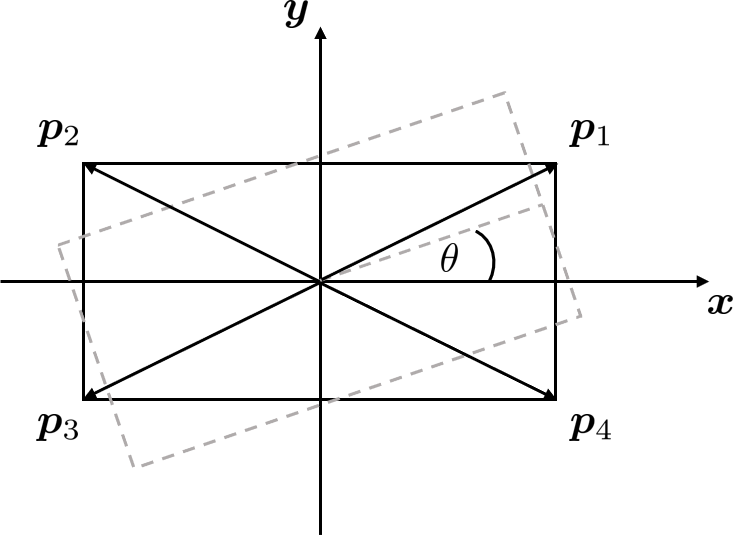
\includegraphics[scale=.5]{chapters/03_background/img/foot_convex_hull.png}
	\caption{The foot's support polygon, which is described by the position vectors $\bm{p}_i$.}
	\label{fig::312_foot_hull}
\end{figure}
A point $\bm{x}$ lies beneath the line that connects the edges if
\begin{align}
	\bm{A}_k^L\bm{x} \leq \bm{B}_k^L,
	\label{eq::312_lin}
\end{align}
where the linear equations are defined by  $\bm{A}_k^L=\begin{pmatrix}
\bm{A}_k^{L,x}\,\bm{A}_k^{L,y}\end{pmatrix}\in\mathbb{R}^{N_{\text{edges}}\times2}$, and $\bm{B}_k^L\in\mathbb{R}^{N_{\text{edges}}\times1}$
\begin{align}
	\bm{A}_k^{L,x}[i] &= p^{L,y}_i-p^{L,y}_{i+1} \\
	\bm{A}_k^{L,y}[i] &= p^{L,x}_{i+1}-p^{L,x}_i \\
	\bm{B}_k^L[i] &= (p^{L,y}_i-p^{L,y}_{i+1})p^{L,x}_{i+1} + (p^{L,x}_{i+1}-p^{L,x}_i)p^{L,y}_{i+1}
\end{align}
Since we require the zero moment point to lie inside the support polygon, $\bm{x}$ in equation \ref{eq::312_lin} is replaced by $\bm{R}_z(f_k^\theta)(\bm{z}_k-\bm{f}_k)$, with $\bm{z}_k=\begin{pmatrix}
z_k^x & z_k^y
\end{pmatrix}^T$, and $\bm{f}_k=\begin{pmatrix}
f_k^x & f_k^y
\end{pmatrix}^T$. This expression describes the zero moment point with respect to the foot frame, where $\bm{R}_z(f_k^\theta) = \begin{pmatrix}
\quad\cos f_k^\theta & \sin f_k^\theta \\
-\sin f_k^\theta& \cos f_k^\theta
\end{pmatrix}$ is an inverse rotation around the z-axis that adds non-linearities to the constraints. We can now extend the formalism to the whole preview horizon by utilizing equations \ref{eq::312_zmp} and \ref{eq:312_feet}. This leads to (\href{https://github.com/mhubii/nmpc_pattern_generator/blob/5a213044c927dc6aac9f7e32ce1e5fb472cd67bb/libs/pattern_generator/src/base_generator.cpp#L946}{link})
\begin{align}
	&\bm{D}_{k+1}(\bm{F}_{k+1}^{\theta})\begin{pmatrix}
		\bm{Z}_{k+1}^x - \bm{F}_{k+1}^x \\
		\bm{Z}_{k+1}^y - \bm{F}_{k+1}^y
	\end{pmatrix} \leq \bm{B}_{k+1} \\
	&\bm{D}_{k+1}(\bm{F}_{k+1}^{\theta})\begin{pmatrix}
		\bm{P}_{zs} \bm{c}_k^x + \bm{P}_{zu}\dddot{\bm{C}}_k^x - \bm{v}_{k+1}f_k^x-\bm{V}_{k+1}\tilde{\bm{F}}_{k+1}^x \\
		\bm{P}_{zs} \bm{c}_k^y + \bm{P}_{zu}\dddot{\bm{C}}_k^y - \bm{v}_{k+1}f_k^y-\bm{V}_{k+1}\tilde{\bm{F}}_{k+1}^y
	\end{pmatrix} \leq \bm{B}_{k+1}
	\label{eq::312_cop_hull}
\end{align}
where $\bm{D}_{k+1}$ depends on $\bm{F}_{k+1}^{\theta} = \bm{P}_{ps}f_k^\theta + \bm{P}_{pu}\bm{F}_{k+1}^\theta$, and holds all the linear equations on the whole preview horizon $\bm{D}_{k+1} = \begin{pmatrix}
	\bm{A}_{k+1}^{L,x}&                  &0                 &\bm{A}_{k+1}^{L,y}&      &0 \\
	                  &\ddots            &                  &                  &\ddots& \\
	0                 &                  &\bm{A}_{k+N}^{L,x}&0                 &      &\bm{A}_{k+N}^{L,y}
\end{pmatrix}$, and $\bm{B}_{k+1}=\begin{pmatrix}
	\bm{B}_{k+1}^L & \dots & \bm{B}_{k+N}^L
\end{pmatrix}^T$. Whether the left foot's or the right foot's convex hull is chosen depends on the support foot at the respective preview interval $k$. Equation \ref{eq::312_cop_hull} can now be expressed in terms of the free variables $\bm{U}_k$ by
\begin{align}
	\bm{D}_{k+1}\begin{pmatrix}
		\bm{P}_{zu} & -\bm{V}_{k+1} & \bm{0} & \bm{0} & \bm{0} & \bm{0}\\
		\bm{0} & \bm{0} & \bm{P}_{zu} & -\bm{V}_{k+1} & \bm{0} & \bm{0}
	\end{pmatrix}\bm{U}_k \leq \bm{B}_{k+1} + \bm{D}_{k+1}\begin{pmatrix}
		-\bm{P}_{zs}\bm{c}_k^x + \bm{v}_{k+1}f_k^x\\
		-\bm{P}_{zs}\bm{c}_k^y + \bm{v}_{k+1}f_k^y
	\end{pmatrix}
\end{align}
The above derivation balance constraints deliver a nice framework, which can be used to express the feasibility constraints as well.
\paragraph{Feasibility Constraints}
The feasibility constraints constrain the foot positioning to areas that the robot of interest can actually reach.  
\paragraph{Obstacle Constraints}
\cite{herdt2010walking} % walking without thinking
\cite{naveau2016reactive} % nmpc for constraint stuff
\subsubsection{The Gauss-Newton Formulation}